% !TeX spellcheck = it_IT
\newpage
\section{Datacenter}
Vediamo alcuni esempi di datacenter:
\begin{example}[Google]
	Il datacenter di \hyperref{https://www.youtube.com/watch?v=avP5d16wEp0&list=LLe8YQrC8Io0iIj1IsacdJRA}{}{}{Google} ha impiegati presenti 24h/24h, una sala dedicata al \textit{networking}, un intero piano di server e uno dedicato al \textbf{raffreddamento}.
\end{example}
\begin{example}[UniPi]
	La rete dell'università di Pisa si compone di più di $9000km$ di fibra con una velocità di connessione tra i datacenter (DCI) di $400 Gbit/s$. Inoltre non ha \textbf{Single Point of Failure} ed è ridondante sia a livello fisico che ai livelli L1 e L2.\\
	Il datacenter principale di San Piero a Grado si costituisce di circa 700 nodi e sfrutta un raffreddamento di tipo \textbf{adiabatico}, ovvero sfrutta l'evaporazione dell'acqua per raffreddare l'ambiente nei momenti più caldi. Ha un \textbf{PUE} di 1.2 e una connessione con il \textit{GARR} di $100Gbit/s$.\\
	Utilizza una topologia di tipo \textbf{spine-leaf} per il traffico locale:
	\begin{center}
		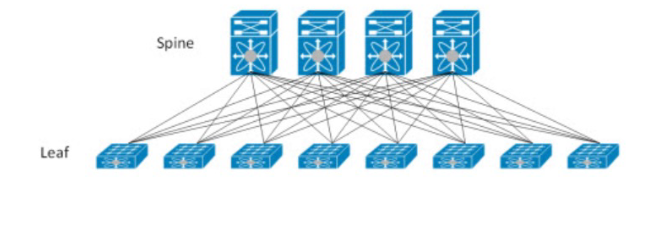
\includegraphics[scale=0.5]{spine_leaf.png}
	\end{center}
\end{example}

\subsection{Energia}
\subsubsection{Consumi}
Nel 2022 i consumi globali dei datacenter sono stati di $460TWh$, circa il $2\%$ del consumo globale, ed è previsto che arrivino a più di $1000TWh$ nel 2026 (il consumo del Giappone).\\
Di tutta questa energia il $40\%$ serve per il \textbf{raffreddamento}.\\
Il posto con la maggiore densità di datacenter è l'Arizona in quanto il costo dell'elettricità è molto basso. Questo perché l'energia usata non è pulita e abbiamo di conseguenza un grosso impatto ambientale.
\subsubsection{PUE}
Il \textbf{Power Usage Effectiveness} misura quanta energia viene usata per componenti non IT all'interno del datacenter (e.g. raffreddamento).
\begin{equation}
	PUE=\frac{P_{IT}+P_{non\_IT}}{P_{IT}} = 1 + \frac{P_{non\_IT}}{P_{IT}}
\end{equation}
\begin{note}
	Il PUE non rappresenta il tasso di energia rinnovabile utilizzata.
\end{note}
\subsection{Management}
La gestione di un datacenter si divide in diversi aspetti:
\begin{itemize}
	\item \textbf{Pianificazione}
	\item \textbf{Installazione} dei rack e delle connessioni
	\item \textbf{Cablaggio}
	\item \textbf{Monitoraggio} dell'infrastruttura
\end{itemize}
\subsubsection{DCIM}
Il \textbf{Data Center Infrastructure Management} si occupa di monitorare in maniera centralizzata l'infrastruttura fisica, in particolare:
\begin{itemize}
	\item Energia
	\item Raffreddamento
	\item Sicurezza
	\item Ambiente
\end{itemize}
Inoltre genera dei \textbf{report} personalizzati e avvisa istantaneamente in caso di \textbf{problemi} all'infrastruttura.
\subsubsection{Sicurezza}
Di seguito alcune cose da \textbf{NON} fare per evitare problemi nel datacenter:
\begin{itemize}
	\item Cavi mal installati
	\item Portare cibi e bevande
	\item Scarsa documentazione
	\item Non tenere traccia di chi ha gli accessi e di quando questi avvengono
	\item Ignorare i rischi di blackout
\end{itemize}
\subsubsection{Outages}
Quando avviene un'interruzione del servizio è importante:
\begin{enumerate}
	\item Essere subito disponibili e concentrati
	\item Gestire bene il panico
	\item Seguire le \textbf{checklist}
\end{enumerate}
Le \textbf{checklist} sono importanti per assicurare \textbf{qualità} nella gestione dell'emergenza e per ridurre la \textbf{responsabilità} dei dipendenti.
\begin{example}[Checklist]
	Un esempio di checklist in caso di incendio:
	\begin{enumerate}
		\item Capire la natura e l'estensione dell'incendio
		\item Usare i sistemi di antincendio a disposizione e se è troppo grosso chiamare subito le autorità ed evacuare
		\item Chiamare le autorità
		\item Evacuare
		\item Se presenti attivare le misure di backup
		\item Appena l'incendio è spento, quantificare i danni
		\item Aggiornare i superiori sulla situazione
	\end{enumerate}
\end{example}

\subsubsection{Continuità e recupero}
Di seguito alcune regole di base per garantire la \textbf{Business Continuity \& Disaster Recovery}:
\begin{itemize}
	\item Mantenere una copia completa dei dati critici almeno a 200km e su una rete elettrica separata
	\item Testare il piano BC/DC
	\item Assicurarsi che eventuali modifiche alla produzione si riflettano sul piano BC/DC
	\item Rendere il piano accessibile e disponibile anche in caso di problemi grossi
	\item Addestrare diverse persone ad eseguire il piano
	\item Ricordare che se qualcosa può andare storto, lo farà
\end{itemize}
\subsection{Iperconvergenza}
Un'infrastruttura può variare in base a quanto vengono virtualizzate le varie parti necessarie (network, server e storage). Ci sono tre casi:
\begin{itemize}
	\item \textbf{Non convergente}: la struttura tradizionale
	\item \textbf{Convergente}: storage e server su macchine separate
	\item \textbf{Iperconvergente}: tutto su un'unica macchina virtualizzata
\end{itemize}
\begin{center}
	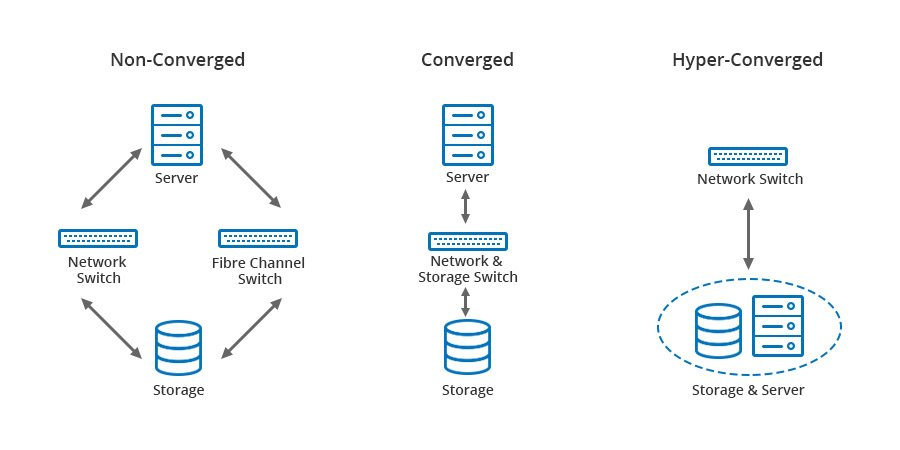
\includegraphics[scale=0.5]{Hyperconvergence.jpg}
\end{center}